% -*- coding:utf-8 -*-
\documentclass[10pt,aspectratio=169,mathserif]{beamer}
% 设置为 Beamer 文档类型,10pt,16:9,数学字体 serif

%%%%-----导入宏包-----%%%%
\usepackage{zju}            % ZJU 模板
\usepackage{ctex}           % 中文支持
\usepackage{amsmath,amsfonts,amssymb,bm}
\usepackage{color}
\usepackage{graphicx,hyperref,url}
\usepackage{metalogo}
\usepackage{fontspec}
\usepackage{xeCJK}
\usepackage{listings}
\usepackage{verbatim} % For verbatim environment

% 解决 macOS 字体警告,使用蘋方字体
% \setCJKmainfont{PingFang SC}
% \setCJKsansfont{PingFang SC}
% \setCJKmonofont{PingFang SC}


\beamertemplateballitem      % 主题

% 版式与溢出优化
\setbeamersize{text margin left=0.8em, text margin right=0.8em}
\setlength{\emergencystretch}{3em}

% listings:Solidity 语言与全局样式
\lstdefinelanguage{Solidity}{
	morekeywords={pragma, solidity, contract, interface, library, using, for, struct, enum, mapping,
		function, event, modifier, return, returns, import, as, is, try, catch, new, emit, require,
		if, else, while, for, do, revert, assembly, unchecked,
		address, string, bytes, bytes1, bytes2, bytes3, bytes4, bytes5, bytes6, bytes7, bytes8, bytes9,
		bytes10, bytes11, bytes12, bytes13, bytes14, bytes15, bytes16, bytes17, bytes18, bytes19,
		bytes20, bytes21, bytes22, bytes23, bytes24, bytes25, bytes26, bytes27, bytes28, bytes29,
		bytes30, bytes31, bytes32, bool, uint, uint8, uint16, uint32, uint64, uint128, uint256,
		int, int8, int16, int32, int64, int128, int256,
		memory, storage, calldata, view, pure, payable, nonReentrant, external, public, internal, private},
	sensitive=true,
	morecomment=[l]{//},
	morecomment=[s]{/*}{*/},
	morestring=[b]",%
}

% 优化 listings 样式以防止溢出
\lstset{
	language=Solidity,
	basicstyle=\ttfamily\scriptsize, % Use smaller font size
	keywordstyle=\color{blue}\bfseries,
	commentstyle=\color{gray},
	stringstyle=\color{teal},
	breaklines=true,         % Enable line breaking
	breakatwhitespace=true,  % Break lines at whitespace
	showstringspaces=false,
	columns=fullflexible,
	tabsize=2,
	keepspaces=true,
	numbers=left,
	numberstyle=\tiny\color{gray},
	frame=single,
	rulecolor=\color{gray!50}
}

% 简易 Go 语言高亮(用于路由/监听示例)
\lstdefinelanguage{Go}{
	morekeywords={package,import,func,return,if,else,for,range,struct,interface,type,map,chan,go,select,case,break,continue,const,var},
	sensitive=true,
	morecomment=[l]{//},
	morestring=[b]",
}

% Bash/Shell 语言高亮(用于命令行示例)
\lstdefinelanguage{Bash}{
	morekeywords={if,then,else,elif,fi,for,do,done,while,until,case,esac,function,return,exit,break,continue,source,export,alias,unset,cd,ls,pwd,mkdir,rm,cp,mv,chmod,chown,grep,sed,awk,sort,uniq,wc,head,tail,cat,echo,printf,read,test,true,false},
	sensitive=true,
	morecomment=[l]{\#},
	morestring=[b]",
	morestring=[b]',
	moredelim=[s][\color{red}]{\$\{}{\}},
	moredelim=[s][\color{red}]{\$(}{)},
	literate={\\}{{\textbackslash}}1
		{--}{{\texttt{-{}-}}}2
		{-}{{\texttt{-}}}1
}

%%%%------------------------%%%%%
\catcode`\。=\active
\newcommand{。}{.}           % 科技文献句号用圆点
%%%%%%%%%%%%%%%%%%%%%

%%%%----首页信息设置----%%%%
\title[DeSci 去中心化科研平台]{DeSci 去中心化科研平台 · 区块链部分演示}
\subtitle{架构设计 · 合约实现 · 测试验证 · 链下集成}

\author[周子为 · 张家畅]{
	周子为(架构设计 · 链下实现 · 后端集成) \\\medskip
	张家畅(合约设计 · 模块实现 · 演示讲解) \\\medskip
	{\small \url{https://github.com/zzw4257/De-Sci-hardhat}}
}

\institute[浙江大学]{
	计算机学院 \\ 浙江大学
}

\date[2025]{\today}

\begin{document}

% 标题页
\begin{frame}
	\titlepage
\end{frame}

% 提纲
\section*{提纲}
\begin{frame}
	\frametitle{提纲}
	\tableofcontents
\end{frame}

%============================
% 1. 背景与架构总览 (周子为)
%============================

\section{背景与架构总览 (周子为)}

\begin{frame}{问题驱动:为何需要 DeSci 平台?}
    \begin{columns}[T]
        \begin{column}{0.48\linewidth}
            \begin{block}{当前科研协作的痛点}
                \begin{itemize}
                    \item \textbf{确权与归属模糊}:贡献难以精确、透明地记录与追溯。
                    \item \textbf{评审周期漫长且不透明}:中心化期刊评审流程效率低下,存在偏见。
                    \item \textbf{影响力量化单一}:过度依赖期刊因子,忽视数据、代码、评审等贡献。
                    \item \textbf{数据孤岛与可复现性危机}:科研数据难以共享,成果难以验证。
                \end{itemize}
            \end{block}
        \end{column}
        \begin{column}{0.48\linewidth}
            \begin{block}{我们的解决方案:基于区块链的信任机器}
                \begin{itemize}
                    \item \textbf{不可篡改的确权}:成果与数据哈希上链,利用 NFT 固化所有权。
                    \item \textbf{透明的同行评审}:评审流程与结果上链,可追溯、可验证。
                    \item \textbf{多维度的影响力}:算法化、可组合的影响力模型,激励多元贡献。
                    \item \textbf{事件驱动的数据协同}:链上事件作为"事实来源",驱动链下数据同步与服务。
                \end{itemize}
            \end{block}
        \end{column}
    \end{columns}
    \begin{alertblock}{核心思想}
        用智能合约固化"规则与事实",用事件驱动"链上与链下"协同,构建一个开放、可信、可组合的去中心化科研协作网络。
    \end{alertblock}
\end{frame}

\begin{frame}{架构概览:10 个核心合约的协同网络}
	\small
    \textbf{设计理念}:\textbf{模块化、可组合、可扩展}。我们将平台功能解耦为 10 个专注的合约,通过一个中心协调器 (`DeSciPlatform`) 进行交互和激励分发。
	\begin{block}{四大核心功能组}
	  \begin{itemize}
	      \item \textbf{平台基础 (2)}: `DeSciRegistry` (身份与角色), `DeSciPlatform` (协调与激励)。
	      \item \textbf{科研资产 (2)}: `ResearchNFT` (成果确权), `DatasetManager` (数据管理)。
	      \item \textbf{验证与约束 (4)}: `ZKPVerifier`, `ZKProof`, `ResearchDataVerifier`, `ConstraintManager` (数据真实性与隐私保护)。
	      \item \textbf{价值与影响力 (2)}: `InfluenceRanking` (多维声誉), `DataFeatureExtractor` (数据价值评估)。
	  \end{itemize}
	\end{block}

	% [图2: 10个核心合约关系图]
    \centering
	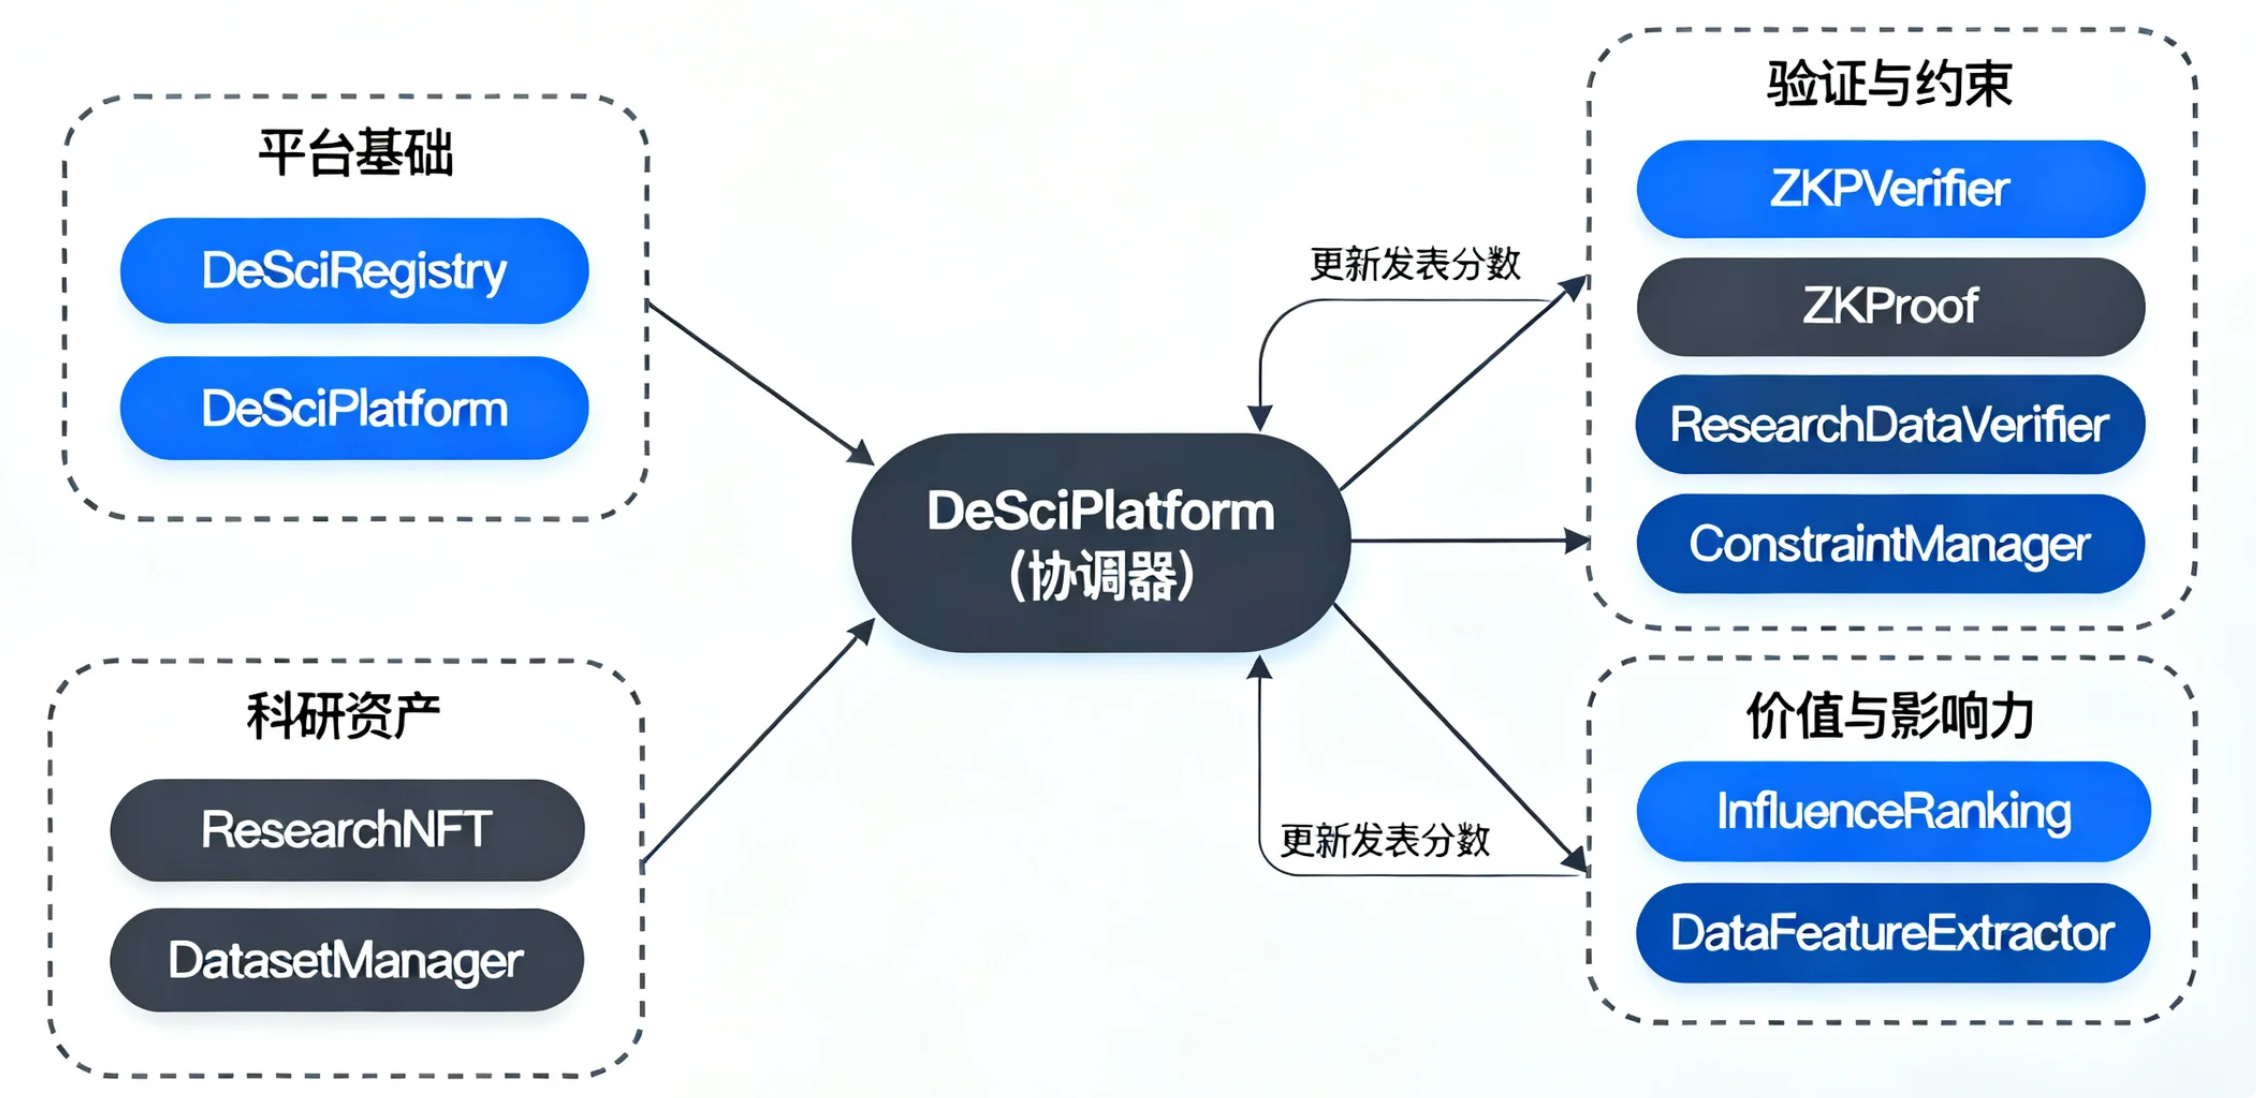
\includegraphics[width=0.4\linewidth]{res/contracts-overview.png}
\end{frame}

\begin{frame}{核心机制:事件驱动的链上写、链下读}
\small
\begin{itemize}
	\item \textbf{链上写 (Write On-Chain)}:
	\begin{itemize}
		\item 用户通过前端与智能合约交互,执行关键操作(如发表、评审)。
		\item 合约内部 \textbf{只存储状态哈希、关键标识符和所有权关系},以降低 Gas 成本。
		\item 操作成功后,合约 \textbf{发射(Emit)包含详细参数的事件},作为不可篡改的日志。
	\end{itemize}
	\item \textbf{链下读 (Read Off-Chain)}:
	\begin{itemize}
        \item \textbf{Go 后端服务}持续监听(Subscribe)区块链上的合约事件。
        \item 监听到新事件后,解析其数据,并将其结构化地存入 \textbf{PostgreSQL 数据库}。
		\item 数据库建立高效索引,支持复杂查询、聚合和分析。
		\item 前端通过 \textbf{RESTful API} 从后端高效读取数据,获得丰富的用户体验。
	\end{itemize}
\end{itemize}
\begin{alertblock}{优势}
兼顾了区块链的\textbf{数据一致性}与\textbf{可信性},以及传统后端的\textbf{高性能}、\textbf{低成本}与\textbf{查询灵活性}。
\end{alertblock}
\end{frame}

%============================
% 2. 合约分组深度解析 (张家畅)
%============================
\section{合约分组深度解析 (张家畅)}

\subsection{组一:科研资产的确权与管理}
\begin{frame}{资产合约: `ResearchNFT` \& `DatasetManager`}
    \begin{columns}[T]
        \begin{column}{0.5\linewidth}
            \textbf{ResearchNFT.sol}
            \begin{itemize}
                \item \textbf{功能}: 科研成果(论文、专利等)铸造为 ERC721 NFT。
                \item \textbf{核心设计}:
                \begin{itemize}
                    \item 支持多作者及其贡献份额。
                    \item 内置同行评审与引用追踪机制。
                    \item 收益分配逻辑(版税、访问费)。
                    \item 内容哈希 (IPFS) 上链,确保数据完整性。
                \end{itemize}
            \end{itemize}
        \end{column}
        \begin{column}{0.5\linewidth}
            \textbf{DatasetManager.sol}
            \begin{itemize}
                \item \textbf{功能}: 数据集的确权、管理与访问控制。
                \item \textbf{核心设计}:
                \begin{itemize}
                    \item 灵活的访问控制 (`AccessType`: 公开/付费/私有)。
                    \item 数据质量等级 (`QualityLevel`),可由授权方更新。
                    \item 与 `InfluenceRanking` 联动,数据被引用可增加贡献者影响力。
                \end{itemize}
            \end{itemize}
        \end{column}
    \end{columns}
    \begin{block}{设计权衡:成本 vs. 功能完备性}
        我们将元数据(如标题、摘要)直接存入事件日志,而非合约存储,显著降低了铸造成本。完整数据存储于 IPFS,链上只保留哈希作为"指针"和"锚点"。
    \end{block}
\end{frame}

\subsection{组二:验证与隐私保护的技术栈}
\begin{frame}{验证合约: `ZKPVerifier`, `ConstraintManager` 等}
	\begin{itemize}
		\item \textbf{目标}: 在保护隐私的同时,验证科研数据的特定属性(如数据符合某个统计分布、实验结果可复现等)。
		\item \textbf{组件协同工作流程}:
		\begin{enumerate}
			\item \textbf{`ResearchDataVerifier`}:作为数据验证的入口,记录待验证数据的哈希。
			\item \textbf{`DataFeatureExtractor`}:(链下执行) 提取数据特征,将特征哈希提交上链。
			\item \textbf{`ConstraintManager`}:定义动态验证规则(如"标准差必须小于 5"),链上可评估特征是否满足约束。
			\item \textbf{`ZKProof` \& `ZKPVerifier`}:对于需要隐私保护的验证,用户提交零知识证明,`ZKPVerifier` 使用预设的 Groth16 验证密钥进行链上验证,不暴露原始数据。
		\end{enumerate}
	\end{itemize}
	\begin{alertblock}{技术亮点}
	    通过组合"公开特征验证"和"零知识证明验证",我们为不同隐私和验证需求提供了分层、灵活的解决方案。
	\end{alertblock}
\end{frame}

\subsection{组三:影响力与激励机制}
\begin{frame}{价值合约: `InfluenceRanking` \& `DeSciPlatform`}
    \begin{columns}[T]
        \begin{column}{0.5\linewidth}
            \textbf{InfluenceRanking.sol}
            \begin{itemize}
                \item \textbf{功能}: 计算用户的多维度影响力分数。
                \item \textbf{核心算法}:
                \begin{itemize}
                    \item \textbf{多维度加权}: 综合发表、评审、数据贡献、协作和治理五个维度的得分。
                    \item \textbf{时间衰减}: 引入时间衰减因子,确保影响力模型的时效性。
                    \item \textbf{可配置权重}: 平台治理可调整各维度权重。
                \end{itemize}
            \end{itemize}
        \end{column}
        \begin{column}{0.5\linewidth}
            \textbf{DeSciPlatform.sol}
            \begin{itemize}
                \item \textbf{功能}: 平台的总协调器和激励中心。
                \item \textbf{核心职责}:
                \begin{itemize}
                    \item \textbf{聚合操作}: 提供 `...WithReward` 函数,将注册、发表等操作与代币奖励原子化绑定。
                    \item \textbf{权限管理}: 作为合约间的"信任根",管理各模块的调用权限。
                    \item \textbf{平台统计}: 聚合关键指标(总用户数、总成果数等)。
                \end{itemize}
            \end{itemize}
        \end{column}
    \end{columns}
\end{frame}

%============================
% 3. 测试验证与工程实践 (共同)
%============================
\section{测试验证与工程实践 (共同)}

\begin{frame}{完备的测试策略:从单元到端到端}
    \begin{block}{测试金字塔}
    \begin{itemize}
        \item \textbf{单元测试 (Unit Tests)}:
        \begin{itemize}
            \item \textbf{覆盖范围}: 每个合约的独立功能、边界条件、权限控制。
            \item \textbf{工具}: Mocha \& Chai。
            \item \textbf{示例}: `DeSciRegistry.test.js` 验证用户注册逻辑和角色权限。
        \end{itemize}
        \item \textbf{集成测试 (Integration Tests)}:
        \begin{itemize}
            \item \textbf{覆盖范围}: 跨合约的完整业务流程。
            \item \textbf{核心文件}: \textbf{`CompleteContractTest.js`}, 验证从用户注册 -> 上传数据集 -> 发表成果 -> 同行评审 -> 影响力更新的全过程。
            \item \textbf{价值}: 确保了 10 个合约作为一个整体能够正确协同工作。
        \end{itemize}
        \item \textbf{端到端测试 (E2E Tests)}:
        \begin{itemize}
            \item \textbf{覆盖范围}: 模拟真实用户场景,包括前端交互、后端API调用和链上状态变更。
            \item \textbf{工具}: Hardhat 脚本 (`scripts/`) + Go 后端测试。
        \end{itemize}
    \end{itemize}
    \end{block}
\end{frame}

\begin{frame}{关键技术挑战与解决方案:`msg.sender` 代理问题}
    \begin{block}{问题现象}
    \small  在集成测试中,通过 `DeSciPlatform.registerUserWithReward()` 注册用户后,发现用户状态在 `DeSciRegistry` 中并未成功置为 `true`。
    \end{block}
    \begin{columns}[T]
    \begin{column}{0.5\linewidth}
        \small \textbf{根本原因分析}
        \begin{itemize}
            \item \small 用户调用 `DeSciPlatform` 合约。
            \item \small `DeSciPlatform` 再去调用 `DeSciRegistry.registerUser()`。
            \item \small 在 `DeSciRegistry` 合约内部,`msg.sender` 变成了 `DeSciPlatform` 的合约地址,而不是原始的用户地址。
            \item \small 导致用户身份被错误地注册到了平台合约上。
        \end{itemize}
    \end{column}
    \begin{column}{0.5\linewidth}
        \small \textbf{解决方案:代理注册模式}
        \begin{itemize}
            \item \small 在 `DeSciRegistry` 中增加一个有权限控制的 `registerUserFor(address \_user, ...)` 方法。
            \item \small 此方法接受一个 `\_user` 地址作为参数,为指定用户注册。
            \item \small 使用 `ADMIN\_ROLE` 限制只有 `DeSciPlatform` 等授权合约才能调用此方法。
            \item \small `DeSciPlatform` 调用 `registerUserFor` 时,传入 `msg.sender` 作为 `\_user` 参数正确传递了用户身份
        \end{itemize}
    \end{column}
    \end{columns}
    \begin{alertblock}{结论}
    这个问题凸显了在复杂合约交互中对 `msg.sender` 和 `tx.origin` 的深刻理解至关重要。通过严谨的集成测试,我们发现并修复了这一关键的架构缺陷。
    \end{alertblock}
\end{frame}

%============================
% 4. Go 后端实现与链下服务 (周子为)
%============================
\section{Go 后端实现与链下服务 (周子为)}

\begin{frame}{Go 后端:链上数据的"消费者"与"服务者"}
    \begin{columns}[T]
        \begin{column}{0.6\linewidth}
            \begin{block}{后端架构:经典三层模型}
                \begin{itemize}
                    \item \small  \textbf{API Layer (Gin)}: 提供 RESTful 接口,处理 HTTP 请求与响应。
                    \item \small \textbf{Service Layer}: 封装核心业务逻辑,如数据聚合、格式转换。
                    \item \small \textbf{Repository Layer (GORM)}: 负责与 PostgreSQL 数据库交互,实现 CRUD 操作。
                \end{itemize}
            \end{block}
             \begin{block}{核心组件:事件监听器}
                \begin{itemize}
                    \item \small \textbf{技术栈}: `go-ethereum` 库。
                    \item \small \textbf{功能}:
                    \begin{itemize}
                        \item \small 连接以太坊节点 (e.g., Hardhat)。
                        \item \small  订阅多个合约的指定事件。
                        \item \small 支持从历史区块回溯事件。
                        \item \small 优雅地处理重连与错误。
                    \end{itemize}
                \end{itemize}
            \end{block}
        \end{column}

        % \begin{figure}
        %     \centering
        %     \includegraphics[width=0.25\linewidth]{image.png}
        %     \caption{Enter Caption}
        %     \label{fig:placeholder}
        % \end{figure}
        \begin{column}{0.4\linewidth}
            % [图7: Go 后端架构与事件流图]
            \centering
            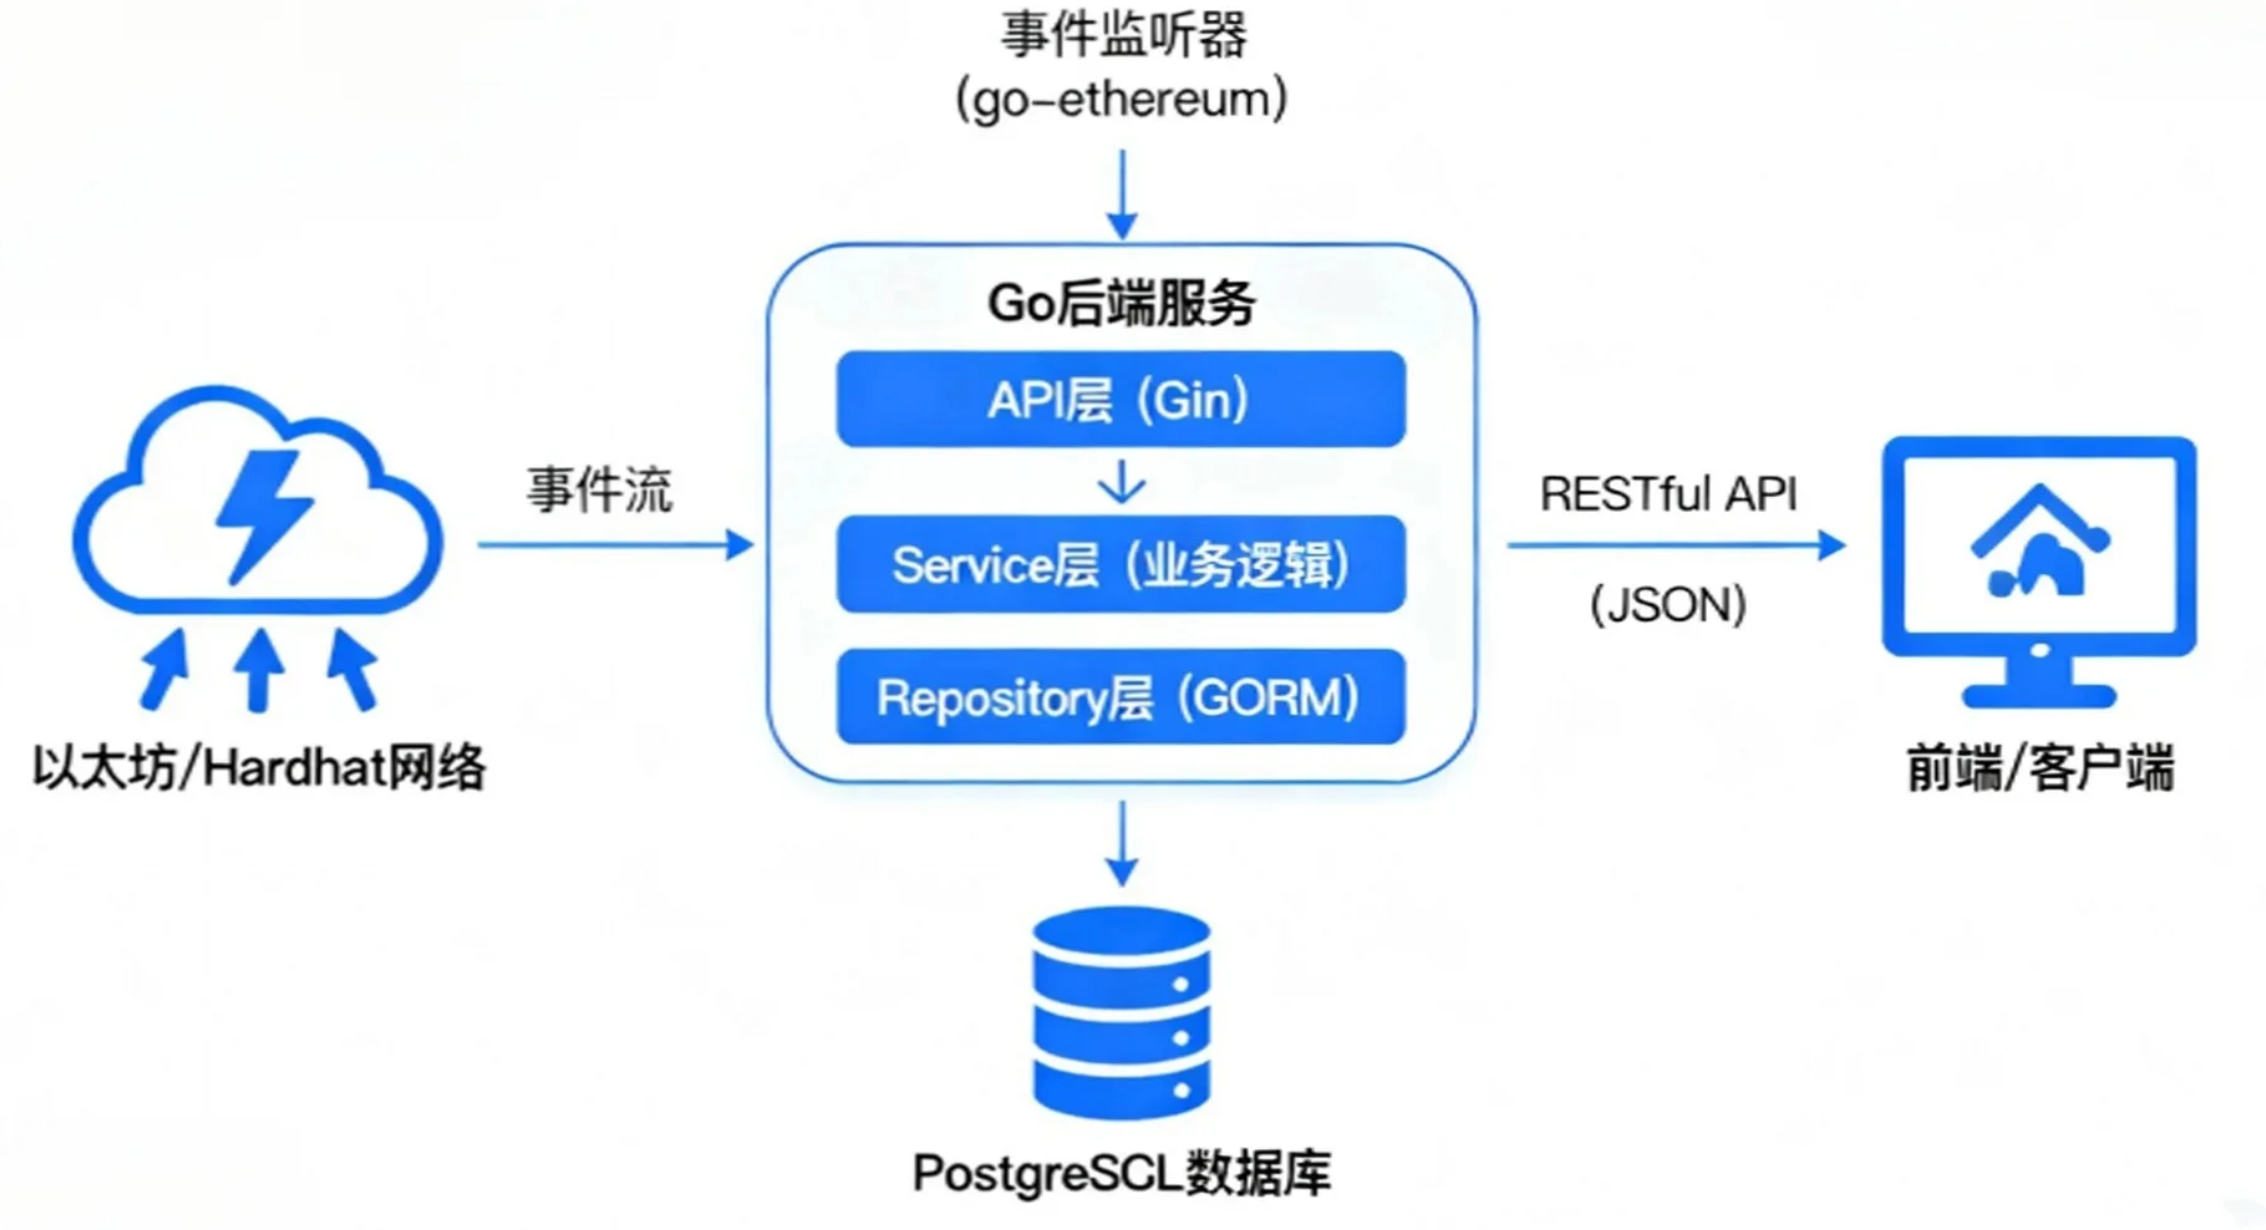
\includegraphics[width=\linewidth]{res/backend-architecture.png}
        \end{column}
    \end{columns}
\end{frame}

%============================
% 5. 系统全景与演示 (张家畅)
%============================
\section{系统全景与演示 (张家畅)}

\begin{frame}{系统全景:区块链在 B/S 架构中的角色}
    这不仅仅是一个"DApp",而是一个将区块链作为核心信任层的现代 Web 服务。
    \begin{itemize}
        \item \textbf{浏览器 (Browser/UI)}: 用户交互界面,通过 MetaMask 等钱包与区块链交互,同时通过 HTTP 请求与后端服务交互。
        \item \textbf{服务器 (Server/Service)}: \textbf{Go 后端},负责提供高性能的读取服务、聚合链上数据、缓存热点数据、处理非关键业务逻辑。
        \item \textbf{区块链 (Blockchain)}: \textbf{Hardhat 网络与智能合约},作为系统的"真理来源"和"规则执行引擎",处理核心的、需要信任的操作。
        \item \textbf{数据层 (Data Layer)}: \textbf{PostgreSQL} (用于索引和查询) + \textbf{IPFS} (用于存储大数据文件)。
    \end{itemize}
\end{frame}

\section{DeSci平台端到端演示}
\begin{frame}
	\frametitle{完整演示流程 - 链上写链下读+数据库集成}
	
	\begin{columns}[c]
		\column{0.5\textwidth}
		\begin{block}{演示步骤}
			\begin{enumerate}
				\item \small \textbf{启动环境} - 部署10个合约到Hardhat
				\item \small \textbf{后端服务} - Go服务连接SQLite+事件监听
				\item \small \textbf{链上交互} - 用户注册、发表研究成果NFT
				\item \small \textbf{链下同步} - 捕获事件并入库SQLite
				\item \small \textbf{数据库验证} - 查询验证数据完整性
				\item \small \textbf{API验证} - RESTful接口获取数据
			\end{enumerate}
		\end{block}
		
		\column{0.5\textwidth}
		\begin{center}
			% 端到端架构图留白
			\fbox{\parbox{0.9\textwidth}{\centering
				\vspace{3cm}
				{\Large \textcolor{blue}{[端到端架构图]}}
				\vspace{0.5cm}
				
				\small 智能合约 → 事件监听 → SQLite → API
				\vspace{0.5cm}
			}}
		\end{center}
	\end{columns}
	
	\vspace{0.3cm}
	\begin{alertblock}{演示重点}
		完整展示链上写、链下读与数据库真实集成的DeSci平台
	\end{alertblock}
\end{frame}

\begin{frame}
	\frametitle{步骤1: 环境启动与合约部署 ��}
	
	\begin{columns}[c]
		\column{0.5\textwidth}
		\begin{block}{启动命令}
			\texttt{\$ npm run deploy-contracts}
		\end{block}
		
		\begin{block}{验证要点}
			\begin{itemize}
				\item Hardhat网络 (Chain ID: 31337) 启动成功
				\item 10个智能合约全部部署完成
				\item 合约地址输出并记录到配置文件
			\end{itemize}
		\end{block}
		
		\column{0.5\textwidth}
\begin{figure}
    \centering
    \includegraphics[width=0.5\linewidth]{部署.png}
    \caption{Enter Caption}
    \label{fig:placeholder}
\end{figure}
	\end{columns}
\end{frame}

\begin{frame}
	\frametitle{步骤2: 后端服务启动与数据库连接 ��}
	
	\begin{block}{启动命令}
		\texttt{\$ cd backend \&\& go run cmd/server/main.go}
	\end{block}
	
	\begin{columns}[c]
		\column{0.5\textwidth}
		\begin{block}{验证要点}
			\begin{itemize}
				\item SQLite数据库连接成功
				\item 区块链事件监听器启动
				\item HTTP API服务器运行 (端口8080)
				\item 合约地址配置加载完成
			\end{itemize}
		\end{block}
		
		\column{0.5\textwidth}
		% 后端启动日志截图留白
		\begin{center}
			\fbox{\parbox{0.9\textwidth}{\centering
				\vspace{2.5cm}
				{\Large \textcolor{blue}{[Go后端启动日志]}}
				\vspace{0.5cm}
				
				\small 
				\texttt{✅ SQLite connected\\
				�� Event listeners started\\
				�� Server running on :8080}
				\vspace{1cm}
			}}
		\end{center}
	\end{columns}
\end{frame}

\begin{frame}
	\frametitle{步骤3: 链上交互与事件触发 ⛓️}
	
	\begin{columns}[c]
		\column{0.5\textwidth}
		\begin{block}{演示脚本}
			\texttt{\$ npx hardhat run scripts/\\
			fullTestScenario.js --network localhost}
		\end{block}
		
		\begin{block}{模拟操作}
			\begin{itemize}
				\item 用户注册 → UserRegistered事件
				\item 上传数据集 → DatasetUploaded事件
				\item 发表研究成果 → ResearchMinted事件
			\end{itemize}
		\end{block}
		
		\column{0.5\textwidth}
		% 链上交互截图留白
		\begin{center}
			\fbox{\parbox{0.9\textwidth}{\centering
				\vspace{2.5cm}
				{\Large \textcolor{orange}{[Hardhat交易日志]}}
				\vspace{0.5cm}
				
				\small 
				\texttt{Transaction: 0xabc123...\\
				ResearchMinted(tokenId: 1)\\
				Gas Used: 234,567}
				\vspace{1cm}
			}}
		\end{center}
	\end{columns}
\end{frame}

\begin{frame}
	\frametitle{步骤4: 链下事件同步与数据库写入 ��}
	
	\begin{block}{事件监听验证}
		Go后端实时捕获链上事件并入库SQLite数据库
	\end{block}
	
	\begin{columns}[c]
		\column{0.5\textwidth}
		\begin{block}{同步过程}
			\begin{itemize}
				\item 监听到ResearchMinted事件
				\item 提取事件参数:tokenId, author, contentHash
				\item 插入到research\_data表
				\item 记录区块号和交易哈希
			\end{itemize}
		\end{block}
		
		\column{0.5\textwidth}
		% 事件同步日志截图留白
		\begin{center}
			\fbox{\parbox{0.9\textwidth}{\centering
				\vspace{2.5cm}
				{\Large \textcolor{purple}{[事件同步日志]}}
				\vspace{0.5cm}
				
				\small 
				\texttt{�� Event Captured: ResearchMinted\\
				�� Inserting to SQLite...\\
				✅ Database sync completed}
				\vspace{1cm}
			}}
		\end{center}
	\end{columns}
\end{frame}

\begin{frame}
	\frametitle{步骤5: SQLite数据库验证 ��️}
	
	\begin{columns}[c]
		\column{0.5\textwidth}
		\begin{block}{数据库查询}
			直接查询SQLite验证数据完整性
		\end{block}
		
		\begin{alertblock}{SQL查询命令}
			\texttt{SELECT * FROM research\_data\\
			WHERE token\_id = '1';}
		\end{alertblock}
		
		\column{0.5\textwidth}
		% 数据库查询截图留白
		\begin{center}
			\fbox{\parbox{0.9\textwidth}{\centering
				\vspace{2.5cm}
				{\Large \textcolor{green}{[SQLite查询结果]}}
				\vspace{0.5cm}
				
				\small
				\texttt{token\_id: 1\\
				title: 区块链科研应用\\
				authors: ["0x123..."]\\
				block\_number: 12345\\
				tx\_hash: 0xabc123...}
				\vspace{0.5cm}
			}}
		\end{center}
	\end{columns}
	
	\vspace{0.3cm}
	\begin{block}{验证要点}
		✅ 链上数据与数据库数据完全一致 \quad ✅ 可追溯性:包含区块号和交易哈希
	\end{block}
\end{frame}

\begin{frame}
	\frametitle{步骤6: RESTful API验证与数据一致性 ��}
	
	\begin{columns}[c]
		\column{0.5\textwidth}
		\begin{block}{API测试}
			通过REST API获取刚才上链的数据
		\end{block}
		
		\begin{alertblock}{测试命令}
			\texttt{curl -X GET \\
			"http://localhost:8080/api/v1/\\
			research/1"}
		\end{alertblock}
		
		\column{0.5\textwidth}
		% API验证截图留白
		\begin{center}
			\fbox{\parbox{0.9\textwidth}{\centering
				\vspace{2.5cm}
				{\Large \textcolor{cyan}{[API响应结果]}}
				\vspace{0.5cm}
				
				\small
				\texttt{\{\\
				"tokenId": "1",\\
				"title": "区块链科研应用",\\
				"authors": ["0x123..."],\\
				"contentHash": "0xabc...",\\
				"blockNumber": 12345\\
				\}}
				\vspace{0.5cm}
			}}
		\end{center}
	\end{columns}
	
	\vspace{0.3cm}
	\begin{block}{一致性验证}
		✅ API数据 = SQLite数据 = 链上数据 \quad ✅ 端到端数据完整性验证成功
	\end{block}
\end{frame}

\begin{frame}
	\frametitle{演示总结 - 数据库真实集成验证 ��}
	
	\begin{columns}[c]
		\column{0.6\textwidth}
		\begin{block}{演示完成验证清单}
			\begin{itemize}
				\item ✅ \textbf{环境部署} - 10个智能合约成功部署
				\item ✅ \textbf{数据库连接} - SQLite真实连接并建表
				\item ✅ \textbf{链上交互} - 用户注册、研究成果发表
				\item ✅ \textbf{事件同步} - 实时捕获并入库SQLite
				\item ✅ \textbf{数据一致性} - 链上链下数据完全一致
				\item ✅ \textbf{API验证} - RESTful接口获取数据库数据
			\end{itemize}
		\end{block}
		
		\begin{alertblock}{核心价值体现}
			完整展示了\textbf{链上写、链下读与数据库真实集成}的DeSci平台架构!
		\end{alertblock}
		
		\column{0.4\textwidth}
		% 数据库集成架构图留白
		\begin{center}
			\fbox{\parbox{0.9\textwidth}{\centering
				\vspace{3cm}
				{\Large \textcolor{red}{[数据库集成架构]}}
				\vspace{0.5cm}
				
				\small 智能合约 → 事件监听 → SQLite → API
				\vspace{1cm}
			}}
		\end{center}
	\end{columns}
\end{frame}
\begin{frame}
    \centering
    \Huge \textbf{感谢聆听}
    \vspace{2em}
    \Large Q \& A
\end{frame}

\end{document}